\begin{frame}[c]
    \frametitle{光子晶体光谱仪}
    \begin{columns}
        \begin{column}{.7\textwidth}
            \begin{itemize}
                \item Pervez, N. K.;  Cheng, W.;  Jia, Z.;  Cox, M. P.;  Edrees, H. M.; Kymissis, I., \textcolor{red}{Photonic crystal} spectrometer. Optics express 2010, 18 (8), 8277-8285.
                \item \textcolor{blue}{创新点:}对阵列响应的确定性控制、小尺寸、计算得到宽带光谱,成本极低。
                \item \textcolor{blue}{意义:}消费者应用,例如彩色印刷和彩色涂料匹配中的监测和反馈。
                \item \footnotesize{该作者还有一篇相似的文章待读:\url{https://doi.org/10.1364/OE.21.004411}}
                \item 使用的材料:聚甲基丙烯酸甲酯(英语:poly (methyl methacrylate),缩写:PMMA)
            \end{itemize}
        \end{column}
        \begin{column}{.3\textwidth}
            \begin{figure}[H] %H为当前位置,!htb为忽略美学标准,htbp为浮动图形
                \centering %图片居中
                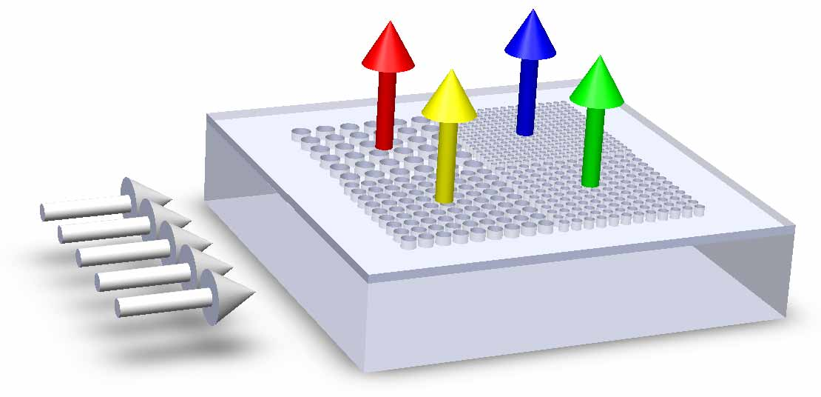
\includegraphics[width=1.\textwidth]{figures/Photonic crystal spectrometer_1.png} %插入图片,[]中设置图片大小,{}中是图片文件名
            \end{figure}
            \begin{figure}[H] %H为当前位置,!htb为忽略美学标准,htbp为浮动图形
                \centering %图片居中
                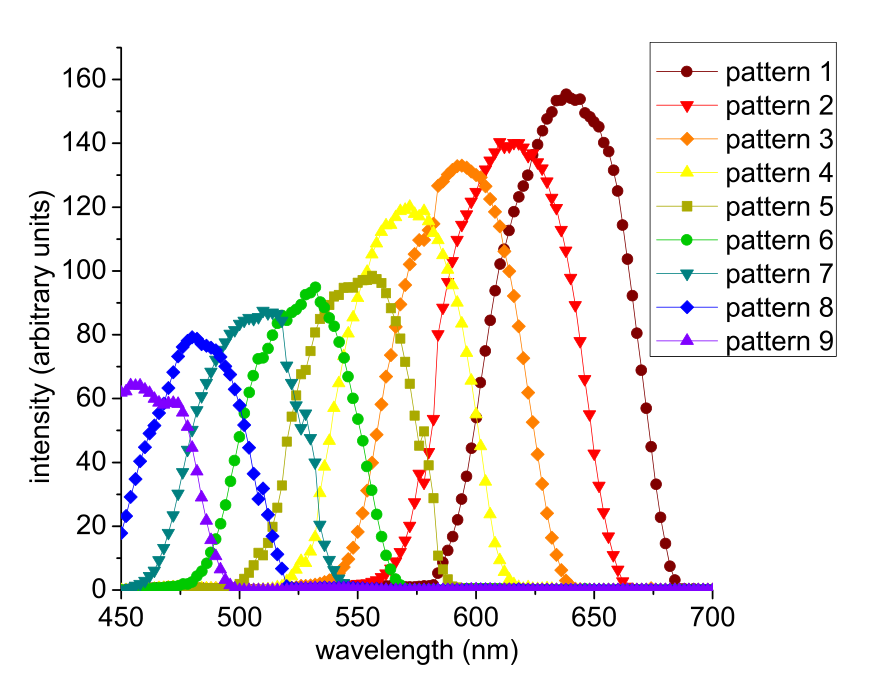
\includegraphics[width=1.\textwidth]{figures/Photonic crystal spectrometer_2.png} %插入图片,[]中设置图片大小,{}中是图片文件名
            \end{figure}
            \begin{figure}[H] %H为当前位置,!htb为忽略美学标准,htbp为浮动图形
                \centering %图片居中
                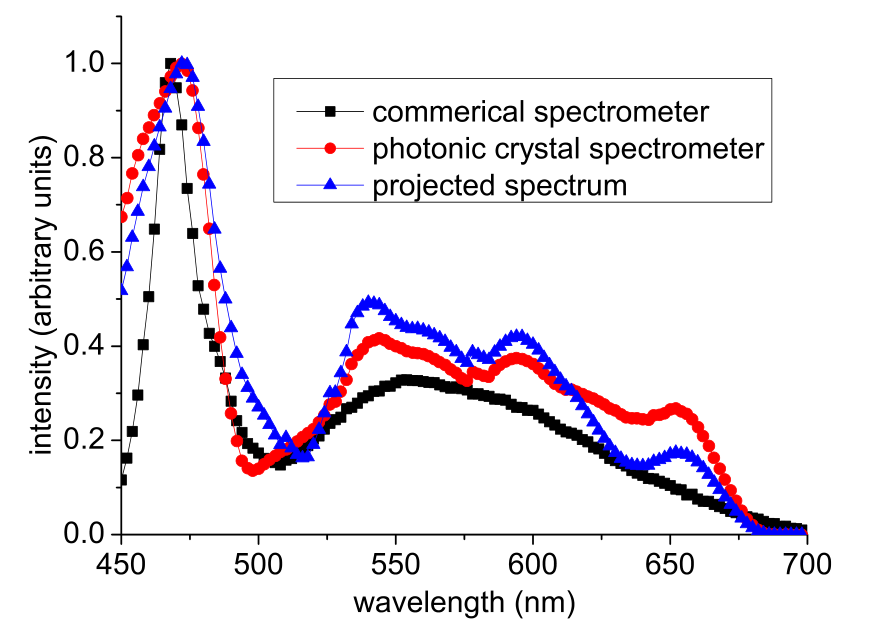
\includegraphics[width=1.\textwidth]{figures/Photonic crystal spectrometer_3.png} %插入图片,[]中设置图片大小,{}中是图片文件名
            \end{figure}
        \end{column}
    \end{columns}
\end{frame}

\begin{frame}[c]
    \frametitle{光子晶体光谱仪}
    \begin{columns}
        \begin{column}{.7\textwidth}
            \begin{itemize}
                \item Pervez, N. K.;  Cheng, W.;  Jia, Z.;  Cox, M. P.;  Edrees, H. M.; Kymissis, I., \textcolor{red}{Photonic crystal} spectrometer. Optics express 2010, 18 (8), 8277-8285.
                \item \textcolor{blue}{机理:}光子晶体由周期性电介质、金属电介质甚至超导体微结构或纳米结构组成,它们影响电磁波传播的方式与半导体晶体中的周期性电势影响电子传播的方式相同,从而确定了允许和禁止的电子能带。光子晶体包含规则重复的高折射率和低折射率区域。
                \item \textcolor{blue}{简化模型:}周期性连续变化的折射率:光子晶体 $\rightarrow$ 周期性离散变化的折射率:薄膜结构
            \end{itemize}
        \end{column}
        \begin{column}{.3\textwidth}
            \begin{figure}[H] %H为当前位置,!htb为忽略美学标准,htbp为浮动图形
                \centering %图片居中
                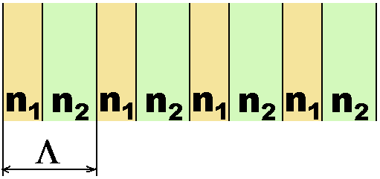
\includegraphics[width=1.\textwidth]{figures/Photonic crystal spectrometer_4.png} %插入图片,[]中设置图片大小,{}中是图片文件名
                \caption{一维光子晶体} %最终文档中希望显示的图片标题
            \end{figure}
            \begin{figure}[H] %H为当前位置,!htb为忽略美学标准,htbp为浮动图形
                \centering %图片居中
                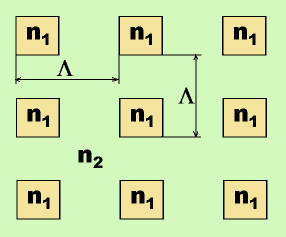
\includegraphics[width=1.\textwidth]{figures/Photonic crystal spectrometer_5.png} %插入图片,[]中设置图片大小,{}中是图片文件名
                \caption{二维光子晶体} %最终文档中希望显示的图片标题
            \end{figure}
            \begin{figure}[H] %H为当前位置,!htb为忽略美学标准,htbp为浮动图形
                \centering %图片居中
                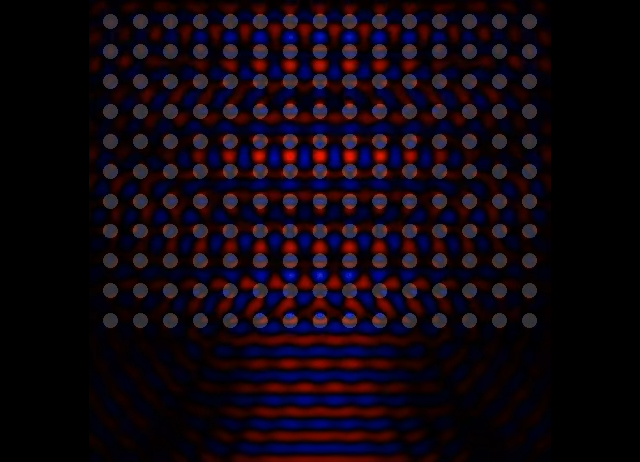
\includegraphics[width=1.\textwidth]{figures/Photonic crystal spectrometer_6.png} %插入图片,[]中设置图片大小,{}中是图片文件名
            \end{figure}
        \end{column}
    \end{columns}
\end{frame}